\documentclass[11pt,letterpaper]{article}
\usepackage[T1]{fontenc}
\usepackage[utf8]{inputenc}
\usepackage{amsmath,amsthm,mathtools}
\usepackage{newtxtext,newtxmath}
\usepackage[margin=1in,headheight=15pt]{geometry}
\usepackage{microtype}
\usepackage{booktabs,array}
\usepackage{xcolor}
\usepackage{tikz}
\usetikzlibrary{arrows.meta}
\usepackage{enumitem}
\usepackage{fancyhdr}
\usepackage{xurl}
\usepackage{hyperref}
\usepackage{cleveref}
\definecolor{inkblue}{HTML}{163A5F}
\definecolor{meshgray}{HTML}{DFE8EF}
\hypersetup{colorlinks=true,linkcolor=inkblue,citecolor=inkblue,urlcolor=inkblue,
  pdftitle={From Mesh Avoidance to Catalan Inflation: A Proof for OEIS A289587},
  pdfauthor={}}
\pagestyle{fancy}
\fancyhf{}
\fancyhead[L]{\small\textsc{Mesh avoidance and Catalan inflation}}
\fancyhead[R]{\small A289587}
\fancyfoot[C]{\small\thepage}
\setlength{\parskip}{3pt}
\setlength{\parindent}{1.2em}
\setlist{itemsep=3pt,topsep=5pt}
\numberwithin{equation}{section}
\newtheorem{theorem}{Theorem}[section]
\newtheorem{lemma}[theorem]{Lemma}
\newtheorem{proposition}[theorem]{Proposition}
\newtheorem{corollary}[theorem]{Corollary}
\theoremstyle{definition}
\newtheorem{definition}[theorem]{Definition}
\newtheorem{example}[theorem]{Example}
\newtheorem{remark}[theorem]{Remark}
\DeclareMathOperator{\Av}{Av}
\DeclareMathOperator{\exc}{exc}
\DeclareMathOperator{\fix}{fix}
\DeclareMathOperator{\occ}{occ}
\DeclareMathOperator{\rec}{rec}
\newcommand{\N}{\mathbb N}
\newcommand{\Q}{\mathbb Q}
\newcommand{\Cat}{\operatorname{Cat}}
\newcommand{\coeff}[2]{[#1^{#2}]}
\newcommand{\Rone}{R_{174}}
\newcommand{\Rtwo}{R_{234}}
\newcommand{\bond}{\operatorname{bond}}
\newcommand{\perma}{\mathcal A}
\newcommand{\permb}{\mathcal B}
\newcommand{\permi}{\mathcal I}
\newcommand{\permd}{\mathcal H}
\allowdisplaybreaks[2]

\title{\color{inkblue}\textbf{From Mesh Avoidance to Catalan Inflation}\\[5pt]
  \large A proof of the generating-function conjecture for OEIS A289587}
\author{A self-contained proof and reproducibility note}
\date{September 20, 2026}

\begin{document}
\maketitle
\thispagestyle{empty}

\begin{abstract}
OEIS A289587 counts permutations avoiding the classical pattern $321$ and
one of two inverse mesh patterns of length two. Its entry attributes an
algebraic generating-function conjecture to Thomas Scheuerle, dated
December 23, 2025. We prove that formula by identifying exactly what a mesh
occurrence means inside a $321$-avoiding permutation. Every occurrence is
either a pair of fixed points or a pair of entries in an increasing run of
consecutive excedance values. Avoidance therefore means at most one fixed
point and no upper succession. Contracting maximal upper-succession runs
is a reversible operation; at the level of the Narayana generating function
it becomes the substitution $u\mapsto u/(1+xu)$. A direct-sum decomposition
then gives the conjectured radical expression. We also derive a full
mesh-occurrence statistic, multivariate refinements, positive coefficient
recurrences and finite sums, an algorithm computing the first $N$ terms with
$O(N)$ integer arithmetic operations, and the precise asymptotic
$a_n\sim 0.4139310680\ldots\,(3.5464554447\ldots)^n n^{-3/2}$ together with
its $1/n$ correction.
The proof is self-contained, and the two accompanying independent
exact-arithmetic programs check the literal mesh definition independently of
the generating function.
\end{abstract}

\vspace{5pt}
\noindent\textbf{Keywords.} Permutation patterns; mesh patterns; Catalan and
Narayana numbers; excedances; fixed points; algebraic generating functions.

\section{The conjecture and the result}
\label{sec:intro}

The classical pattern $321$ occurs in a permutation $\pi=\pi_1\cdots\pi_n$
when there are indices $i<j<k$ with $\pi_i>\pi_j>\pi_k$.
Write $\Av_n(321)$ for the permutations with no such triple. This is a
central Catalan family; the excedance structure and its connection with
lattice paths have been studied in detail, for example by
Reifegerste~\cite{reifegerste}. We will prove the particular facts needed
here rather than assume them.

A mesh pattern adds empty-region conditions to an ordinary pattern.
For the underlying pattern $12$, select $i<j$ with $a=\pi_i<b=\pi_j$.
The vertical lines through $i,j$ and horizontal lines through $a,b$ divide
all other permutation points into nine open rectangles. Label their
columns and rows $0,1,2$, from left to right and from bottom to top.
A pair is an occurrence of $(12,R)$ if every rectangle indexed by
$(c,r)\in R$ is empty. Points on the selected lines cause no ambiguity,
since a permutation has distinct positions and distinct values.
This is the usual mesh-pattern framework of Br\"and\'en and
Claesson~\cite{branden-claesson}, specialized to a length-two pattern.

The shading sets relevant to A289587 are
\begin{align}
 \Rone&=\{(0,1),(0,2),(1,0),(1,2),(2,1)\},\label{eq:Rone}\\
 \Rtwo&=\{(0,1),(1,0),(1,2),(2,0),(2,1)\}.
 \label{eq:Rtwo}
\end{align}
These coordinates agree with the encoding described in the linked SeqFan
thread~\cite{seqfan}, which assigns the cell $(c,r)$ the weight $2^{3c+r}$;
summing the weights of the shaded cells gives the displayed labels $174$
and $234$. Those labels only name the patterns and play no arithmetic role
in the proof. The explicit sets also remove any dependence of our proof or
programs on an unexplained numerical pattern identifier.

\begin{figure}[ht]
\centering
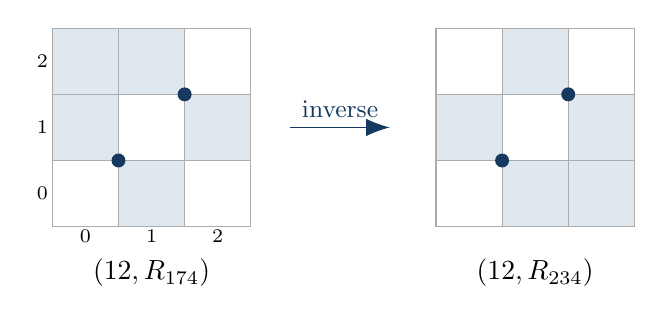
\begin{tikzpicture}[scale=0.84]
 \begin{scope}
  \foreach \x/\y in {0/1,0/2,1/0,1/2,2/1}
   \fill[meshgray] (\x,\y) rectangle +(1,1);
  \draw[step=1,gray!65,thin] (0,0) grid (3,3);
  \fill[inkblue] (1,1) circle (3pt);
  \fill[inkblue] (2,2) circle (3pt);
  \node at (1.5,-0.70) {$(12,R_{174})$};
  \foreach \v in {0,1,2} {
   \node[font=\scriptsize] at (\v+0.5,-0.15) {\v};
   \node[font=\scriptsize] at (-0.15,\v+0.5) {\v};}
 \end{scope}
 \draw[-{Latex[length=3mm]},inkblue] (3.6,1.5)--(5.1,1.5)
  node[midway,above,font=\small] {inverse};
 \begin{scope}[xshift=5.8cm]
  \foreach \x/\y in {0/1,1/0,1/2,2/0,2/1}
   \fill[meshgray] (\x,\y) rectangle +(1,1);
  \draw[step=1,gray!65,thin] (0,0) grid (3,3);
  \fill[inkblue] (1,1) circle (3pt);
  \fill[inkblue] (2,2) circle (3pt);
  \node at (1.5,-0.70) {$(12,R_{234})$};
 \end{scope}
\end{tikzpicture}
\caption{Shaded rectangles must contain no other permutation points.
Transposition of the diagram interchanges the two mesh patterns.}
\label{fig:meshes}
\end{figure}

Let $a_n$ count $\pi\in\Av_n(321)$ avoiding $(12,\Rone)$, including the
empty permutation at $n=0$.

\begin{lemma}[Inverse equivalence]
\label{lem:inverse}
The map $\pi\mapsto\pi^{-1}$ is a bijection between the class of
$321$-avoiders avoiding $(12,\Rone)$ and the class of $321$-avoiders
avoiding $(12,\Rtwo)$.
\end{lemma}
\begin{proof}
Inverting a permutation transposes its point plot. The pattern $12$ is
invariant under transposition, the classical pattern $321$ is its own
inverse, and transposing every cell of $\Rone$ gives exactly $\Rtwo$.
Thus inversion preserves $321$-avoidance and exchanges the two mesh
restrictions, in both directions.
\end{proof}

\noindent
Both versions in the OEIS definition therefore have the same counting
sequence. This equivalence is proved, not inferred from agreement of
initial terms. Refinements by excedances below refer to the $(12,\Rone)$
class; the inverse bijection need not preserve that statistic.

The OEIS entry~\cite{oeis} lists
\[
\begin{gathered}
1,1,1,3,6,18,47,139,405,1225,3740,11602,\\
36357,115049,366969,1178791,3809802.
\end{gathered}
\]
for $n=0,\ldots,16$, and marks the following formula as conjectural.

\begin{theorem}[The A289587 generating function]
\label{thm:main}
Set
\begin{align*}
 D(x)&=x^4-2x^3-5x^2-2x+1,\\
 P(x)&=x^4+4x^3+11x^2+10x+3,\qquad Q(x)=x^2+5x+3.
\end{align*}
Then
\begin{equation}
 \boxed{\displaystyle
 A(x):=\sum_{n\ge0}a_nx^n
   =\frac{P(x)-Q(x)\sqrt{D(x)}}{8x(1+x)^2}.}
 \label{eq:main}
\end{equation}
Here $\sqrt{D(x)}$ is the formal square root with constant term $1$;
the apparent singularity at $x=0$ is removable.
\end{theorem}

The interesting issue is not recognizing a square root from these numbers.
A mesh condition quantifies over two selected entries and the emptiness of
several surrounding rectangles. It can detect arbitrarily distant entries,
and so need not reduce to a local prohibition. Here it does not: besides a
local obstruction there is a genuinely global one, namely two singleton
direct-sum components, even when they are separated by a nontrivial
component. The proof below isolates that obstruction before any
generating-function manipulation is performed.

\paragraph{Status and scope.}
The entry, consulted on September 20, 2026, still labels \eqref{eq:main}
``Conjectured g.f.'' and credits Scheuerle on December 23, 2025.
The proof below establishes the exact identity, not merely an initial
coefficient agreement. I did not locate a proof of this formula in the entry
or its linked discussion. This is a proof of the OEIS-listed conjecture;
we make no claim that an exhaustive literature search has ruled out every
independent prior derivation. Standard Catalan and Narayana ingredients
are explicitly separated from the mesh-specific argument.

\section{Elementary structure of \texorpdfstring{$321$}{321}-avoiders}
\label{sec:structure}

An index $i$ is an \emph{excedance} of $\pi$ if $\pi_i>i$, and a fixed
point if $\pi_i=i$. Let $\exc(\pi)$ and $\fix(\pi)$ denote their numbers.
An entry is a left-to-right maximum if it exceeds every preceding entry.

\begin{lemma}[Two increasing subsequences]
\label{lem:biinc}
In a $321$-avoiding permutation, the entries at excedance positions form
an increasing subsequence, and the entries at nonexcedance positions form
an increasing subsequence. Conversely, these two increasing-subsequence
conditions imply $321$-avoidance. Every excedance entry is a left-to-right
maximum.
\end{lemma}
\begin{proof}
Suppose $i<j$ are excedances with $\pi_i>\pi_j$. Since $\pi_j>j$, not all
values smaller than $\pi_j$ can occupy the first $j-1$ positions.
Some $k>j$ has $\pi_k<\pi_j$, giving a forbidden triple.
The same argument proves the last assertion: if $j$ is an excedance and
an earlier entry is larger than $\pi_j$, a smaller later value completes
a $321$.

Now suppose $i<j$ are nonexcedances with $\pi_i>\pi_j$. There are only
$\pi_i-1$ values below $\pi_i$, and at least one of them, namely $\pi_j$,
is later than position $i$. Because $i\ge\pi_i$, the $i-1$ preceding
positions cannot all contain values below $\pi_i$. Some $h<i$ therefore
has $\pi_h>\pi_i>\pi_j$, again impossible.

For the converse, any three entries include two belonging to the same
one of the two indicated subsequences. Those two entries are increasing,
so the three entries cannot be decreasing.
\end{proof}

\begin{lemma}[A fixed point separates the permutation]
\label{lem:fixed}
If $\pi\in\Av_n(321)$ and $\pi_i=i$, then all earlier values are less
than $i$ and all later values are greater than $i$.
\end{lemma}
\begin{proof}
If an earlier value exceeded $i$, counting the values $1,\ldots,i-1$
would force a later value below $i$. Together with $\pi_i=i$ these would
form a $321$. Thus all $i-1$ preceding values are below $i$; they are
exactly $1,\ldots,i-1$, and every later value is larger.
\end{proof}

For permutations $\alpha$ of length $r$ and $\beta$ of length $s$, their
\emph{direct sum} is
\[
 \alpha\oplus\beta
   =\alpha_1\cdots\alpha_r\,(\beta_1+r)\cdots(\beta_s+r).
\]
A nonempty permutation is sum-indecomposable if it is not a direct sum
of two nonempty permutations. Every permutation has a unique decomposition
into sum-indecomposable blocks: cut precisely after those $j<n$ for which
the first $j$ values form the set $\{1,\ldots,j\}$.

By \cref{lem:fixed}, fixed points of a $321$-avoider are exactly the
singleton blocks in this decomposition. No triple $321$ straddles a
direct-sum boundary, so each block is itself a $321$-avoider.
These facts will make the fixed-point restriction particularly simple.
We use ``fixed point'' and ``singleton direct-sum component''
interchangeably from now on; inside $\Av(321)$ they are the same thing.

The class can also be described using left-to-right maxima instead of
excedances, and the literature on $321$-avoiders uses both. The two
descriptions are not interchangeable as local conditions, and the next
lemma records exactly where they agree. It is used in
\cref{rem:records} and in the second verification program, and nowhere in
the main line of the proof.

\begin{lemma}[Records, excedances and fixed points]
\label{lem:records}
Let $\pi\in\Av_n(321)$ and write $\rec(\pi)$ for its number of
left-to-right maxima. Then:
\begin{enumerate}[label=\upshape(\roman*)]
\item $\pi_i$ is a left-to-right maximum if and only if $i$ is an
  excedance or a fixed point. Hence
  $\rec(\pi)=\exc(\pi)+\fix(\pi)$.
\item A sum-indecomposable $\pi$ of length at least two has no fixed
  point. On such a permutation the left-to-right maxima are exactly the
  excedance entries, so $\rec(\pi)=\exc(\pi)$.
\item If $\pi_i$ is a left-to-right maximum, $\pi_{i+1}=\pi_i+1$, and
  there is a sum cut at $i$, then the entries at positions $i$ and $i+1$
  are two adjacent singleton components.
\item Within a direct-sum component, being a left-to-right maximum is
  equivalent to being one after standardizing that component.
\end{enumerate}
\end{lemma}
\begin{proof}
(i) An excedance entry is a left-to-right maximum by \cref{lem:biinc};
a fixed point is one by \cref{lem:fixed}. Conversely, if $\pi_i$ exceeds
all $i-1$ preceding entries then $\pi_i\ge i$, so $i$ is an excedance or
a fixed point. The two cases are disjoint.

(ii) A fixed point is a singleton block, so an indecomposable permutation
of length at least two has none, and (i) applies.

(iii) A sum cut at $i$ means $\{\pi_1,\ldots,\pi_i\}=\{1,\ldots,i\}$, so
the largest of the first $i$ entries is $i$; since $\pi_i$ is a
left-to-right maximum, $\pi_i=i$ and therefore $\pi_{i+1}=i+1$. Then
$\{\pi_1,\ldots,\pi_{i-1}\}=\{1,\ldots,i-1\}$ and
$\{\pi_1,\ldots,\pi_{i+1}\}=\{1,\ldots,i+1\}$, so $i-1$ and $i+1$ are
sum cuts as well and both entries are singleton components.

(iv) Every earlier component consists of values smaller than every value
of the current one, so it neither creates nor destroys a maximum.
\end{proof}

\section{The exact mesh-occurrence statistic}
\label{sec:mesh}

\begin{definition}
An \emph{upper succession}, also called an upper bond in this note, is a
pair of adjacent positions $i,i+1$ satisfying
\begin{equation}
 \pi_i>i,\qquad \pi_{i+1}=\pi_i+1.
 \label{eq:bond}
\end{equation}
Both positions are then excedances. A maximal upper run is a maximal
consecutive block of excedance entries whose values rise by one at each
step. Excedance entries not belonging to a longer run count as runs of
length one.
\end{definition}

\begin{theorem}[Occurrence formula]
\label{thm:occ}
Let $\pi\in\Av_n(321)$ have $f$ fixed points and maximal upper-run lengths
$\ell_1,\ldots,\ell_k$. Then
\begin{equation}
 \boxed{\displaystyle
 \occ_{(12,\Rone)}(\pi)
   =\binom f2+\sum_{j=1}^k\binom{\ell_j}{2}.}
 \label{eq:occ}
\end{equation}
More precisely, its mesh occurrences are exactly the pairs of fixed points
and the pairs of entries lying in the same maximal upper run.
\end{theorem}
\begin{proof}
For an occurrence with endpoints $(i,a)$ and $(j,b)$, the shading
\eqref{eq:Rone} says exactly that
\begin{align}
 &\pi_h<a &&\text{for every }h<i, \label{eq:left}\\
 &a<\pi_h<b &&\text{for every }i<h<j,\label{eq:middle}\\
 &\pi_h\notin(a,b) &&\text{for every }h>j.\label{eq:right}
\end{align}
Every value strictly between $a$ and $b$ must therefore occur strictly
between positions $i$ and $j$, and every entry in those positions has
such a value. Consequently
\begin{equation}
 j-i=b-a,
 \qquad \{\pi_i,\ldots,\pi_j\}=\{a,a+1,\ldots,b\}.
 \label{eq:interval}
\end{equation}
Also \eqref{eq:left} forces $a\ge i$.

If $a=i$, then \eqref{eq:interval} gives $b=j$: the endpoints are fixed
points. Conversely, any pair of fixed points satisfies
\eqref{eq:left}--\eqref{eq:right} by \cref{lem:fixed}.

If $a>i$, at least one value $c<a$ is missing from the $i-1$ positions
before $i$. It cannot lie between $i$ and $j$ by \eqref{eq:middle}; hence
it lies after $j$. An inversion anywhere in the block from $i$ to $j$,
followed by this value $c$, would create a $321$. The whole block is
therefore increasing, and \eqref{eq:interval} makes it
\[
 a,\ a+1,\ \ldots,\ b.
\]
Every one of these positions is an excedance because the value minus
the position is the constant $a-i>0$. Thus the endpoints lie in one
upper run.

Conversely, take two entries in one upper run. The first is a
left-to-right maximum by \cref{lem:biinc}. All intermediate values occur
consecutively between the endpoints, so none can occur later.
Thus \eqref{eq:left}--\eqref{eq:right} hold. The two types of occurrence
are disjoint, and counting endpoint pairs proves \eqref{eq:occ}.
\end{proof}

\begin{corollary}[The mesh condition without a mesh diagram]
\label{cor:character}
A permutation $\pi\in\Av_n(321)$ avoids $(12,\Rone)$ if and only if
it has no upper succession and has at most one fixed point.
\end{corollary}

This is the decisive step: a condition involving five empty rectangles
has become one local prohibition and one global restriction on singleton
sum blocks. Equivalently, and this is the form in which the criterion is
most often stated, a $321$-avoider \emph{contains} $(12,\Rone)$ exactly
when it has an upper succession or at least two singleton direct-sum
components. \Cref{thm:occ} is strictly stronger: \cref{cor:character} is
its specialization to $\occ=0$.

\begin{remark}[Two local conditions that are not the same condition]
\label{rem:records}
A variant of \eqref{eq:bond} appears naturally if one marks left-to-right
maxima instead of excedances: call $i$ a \emph{record bond} when $\pi_i$
is a left-to-right maximum and $\pi_{i+1}=\pi_i+1$. These are genuinely
different predicates. The permutation $123$ has the record bonds $1,2$
and $2,3$ but no upper succession at all, since every entry is a fixed
point; among the $321$-avoiders of length at most six there are $31$ on
which the two predicates disagree. What is true is the following.
By \cref{lem:records}(i), a record bond that is not an upper succession
starts at a fixed point $\pi_i=i$ and then $\pi_{i+1}=i+1$, which by
\cref{lem:records}(iii) makes both entries singleton components; so a
record bond that is not an upper succession forces a second fixed point.
Hence
\[
 \text{no upper succession and }\fix\le1
 \quad\Longleftrightarrow\quad
 \text{no record bond and }\fix\le1,
\]
and the two conjunctions cut out the same class, even though neither
local condition implies the other. On the nontrivial sum-indecomposable
$321$-avoiders, where the contraction of \cref{sec:core} is actually
performed, \cref{lem:records}(ii) makes the two predicates literally
identical, because there are no fixed points there. This is why the
record-refined and excedance-refined core series of \cref{sec:refinements}
are the same series and not a shift of one another; both descriptions are
correct, and the merged notation below uses excedances throughout.
\end{remark}

\begin{example}
The five $321$-avoiders of length three are
$123,132,213,231,312$. The first has three fixed points, while $231$ has
the upper succession $2,3$. The remaining three are accepted, giving
$a_3=3$. The permutation $1324=1\oplus21\oplus1$ has no upper succession, but its two
fixed points, $1$ and $4$, form a mesh occurrence. Thus the fixed-point
condition cannot be omitted; note that the two singleton blocks producing
it are not adjacent, so banning adjacent singletons would not suffice
either.

By contrast, $4123$ is accepted. Its consecutive ascents $1,2$ and $2,3$
are neither excedance successions nor ascents beginning at a left-to-right
maximum, and it is sum-indecomposable with no fixed point. This is the
example to keep in mind: plain succession-avoidance is the wrong local
condition, and the word ``upper'' in \eqref{eq:bond} is doing real work.
\end{example}

\section{Contracting upper runs}
\label{sec:core}

The next step is an exact decomposition, not an inclusion--exclusion
approximation. Contract every maximal upper run to one entry and
standardize the resulting word, meaning that its smallest remaining
value becomes $1$, the next becomes $2$, and so on. Call the result the
\emph{upper-run core}.

\begin{theorem}[Canonical core and inflation]
\label{thm:core}
Every $321$-avoiding permutation has a unique representation as a
$321$-avoiding core with no upper succession, with each excedance entry
of the core inflated into a nonempty increasing interval. The lengths
of the inflated intervals are precisely the original maximal upper-run
lengths. This operation preserves the number of fixed points and
preserves the direct-sum block structure.
\end{theorem}
\begin{proof}
We first justify a single contraction. Suppose adjacent positions
$i,i+1$ contain $a,a+1$ with $a>i$. Delete the second entry and
standardize. Pattern avoidance survives taking a subpermutation.
All entries before $i$ are below $a$ by \cref{lem:biinc}, so they are
unchanged. The surviving entry $a$ remains an excedance.

For an entry later than $i+1$, if its value is larger than $a+1$, both
its position and value decrease by one; its excedance or fixed-point
status is unchanged. Suppose instead that this later entry is $b<a$
at position $j$. Every value smaller than $b$ must precede $j$:
otherwise $a,b$, and a later smaller value would form a $321$.
The $j-1$ preceding positions contain those $b-1$ smaller values and
also both $a,a+1$. Therefore $j-1\ge b+1$, or $b\le j-2$.
After contraction, $b<j-1$, so it remains a strict nonexcedance.
Thus precisely one excedance disappears, and no fixed point appears or
disappears.

It remains important to check that contraction creates no unexpected
new upper bond. If two consecutive excedance entries have a gap between
their values, every value in that gap occurs later: the first entry is
a left-to-right maximum and there is no position between the two.
Such intervening values cannot be later excedances, since excedance
values increase; they are nonexcedances and are never contracted.
Their presence therefore prevents the gap from disappearing.
Likewise, a nonexcedance between two upper runs is never deleted, so
separated runs cannot become adjacent. Contracting a bond within a
run merely shortens that run. Hence the maximal runs have a uniquely
determined bond-free core, independent of contraction order.

Conversely, inflate any excedance of a bond-free core into a consecutive
increasing block. Increasing interval inflation preserves $321$-avoidance:
a decreasing triple uses at most one entry from such a block, and would
project to a decreasing triple in the core. Entries before the inflated
point have smaller values and are unchanged; later larger entries have
both position and value shifted by the same amount, while later smaller
entries stay strict nonexcedances. Fixed points remain fixed, and all
entries of the inflated block are excedances.

A pre-existing position gap between core excedances contains a retained
nonexcedance; a pre-existing value gap contains a retained nonexcedance
value, by the preceding argument. Hence different inflated blocks never
merge into one upper run. The inflation lengths and the core are
therefore recovered uniquely by contraction.

Finally, an upper bond cannot cross a direct-sum boundary. If it did,
its first value, being a left-to-right maximum and lying in the left
summand, would have to equal the boundary position, contradicting strict
excedance. Inflating an entry of a nontrivial indecomposable block
preserves indecomposability: a sum cut between distinct inflated blocks
would project to a sum cut in the core; a cut inside an inflated block
is impossible because its first entry still exceeds its position and
leaves a smaller value on the right. Thus the sum blocks correspond
under contraction and inflation.
\end{proof}

\begin{example}
The permutation
\[
 2341675=2341\oplus231
\]
has upper runs of lengths $3$ and $2$. Its core is $2143=21\oplus21$.
Inflating the two excedances of $2143$ by those lengths reconstructs
$2341675$. The occurrence formula gives $\binom32+\binom22=4$
mesh occurrences.
\end{example}

\section{The Narayana generating function, from first principles}
\label{sec:narayana}

Define
\begin{equation}
 C(x,u)=\sum_{n\ge0}\ \sum_{\pi\in\Av_n(321)}x^n u^{\exc(\pi)}.
 \label{eq:Cdef}
\end{equation}
We need its functional equation with $u$ still present; substituting the
ordinary Catalan series $C(x,1)$ too early would lose exactly the
information needed for upper-run contraction.

\begin{lemma}[Excedance arrays and Dyck valleys]
\label{lem:dyck}
Permutations in $\Av_n(321)$ with $k$ excedances are in bijection with
Dyck paths of semilength $n$ having $k$ valleys.
\end{lemma}
\begin{proof}
Let $e_1<\cdots<e_k$ be the excedance positions and
$v_1<\cdots<v_k$ their values. By \cref{lem:biinc}, the remaining values
occupy the remaining positions in increasing order. The pair of arrays
therefore determines the permutation, and satisfies $e_j<v_j$.

Conversely, choose increasing arrays in $\{1,\ldots,n\}$ with $e_j<v_j$,
put $v_j$ in position $e_j$, and fill the remaining positions increasingly.
For every $t$, the number of selected positions at most $t$ is at least
the number of selected values at most $t$, since $v_j\le t$ implies
$e_j<t$. Thus the number of unselected values at most $t$ is at least
the number of unselected positions at most $t$. Increasing matching
places each remaining value at a position at least as large as itself.
These are precisely the nonexcedances, and the two increasing
subsequences imply $321$-avoidance.

Use north and east steps for a Dyck path from $(0,0)$ to $(n,n)$ staying
in $y\ge x$. Specify its valleys (an east step followed by a north step)
to be
\[
 (e_1,v_1-1),\ldots,(e_k,v_k-1).
\]
Both coordinates increase strictly, and $e_j\le v_j-1$. These valleys
uniquely determine a path: alternate maximal north and east runs,
starting with a north run and ending with an east run. Each valley is
on or above the diagonal, so the whole path stays above it. Conversely,
the valleys of such a path recover exactly the allowed arrays.
The path with no valleys is $N^nE^n$, corresponding to the identity
permutation.
\end{proof}

\begin{proposition}[Narayana equation]
\label{prop:narayana}
The series $C(x,u)$ is the unique formal solution with constant term $1$
of
\begin{equation}
 C=1+xC(1-u+uC).
 \label{eq:narayana}
\end{equation}
Equivalently, for $n\ge1$,
\begin{equation}
 \coeff{x}{n}\coeff{u}{k}C(x,u)
   =\frac1n\binom nk\binom n{k+1},\qquad 0\le k<n.
 \label{eq:Nnumber}
\end{equation}
\end{proposition}
\begin{proof}
A nonempty Dyck path decomposes uniquely as $NPEQ$, where $P,Q$ are
Dyck paths. There is a new valley between the indicated $E$ and the
start of $Q$ exactly when $Q$ is nonempty. Thus the generating function
is $1+xC(1+u(C-1))$, proving \eqref{eq:narayana}. The factor $x$ determines
each coefficient from earlier ones, giving uniqueness.

For the coefficient formula put $Y=C-1$. Then
$Y=x(1+Y)(1+uY)$. Formal Lagrange inversion~\cite{flajolet-sedgewick} gives
\[
 \coeff{x}{n}Y=\frac1n\coeff{z}{n-1}(1+z)^n(1+uz)^n.
\]
Extracting $u^k$ proves \eqref{eq:Nnumber}. This recovers the classical
Narayana distribution of excedances (cf.\ \cite[Corollary 3.7]{reifegerste})
with the indexing conventions used here.
\end{proof}

\section{From contraction to the conjectured radical}
\label{sec:proof}

Let $B(x,u)$ count all upper-bond-free $321$-avoiders by length and
excedance number, with any number of fixed points. A core excedance
has weight $xu$. Inflating it into a positive run changes this weight to
\[
 xu+(xu)^2+(xu)^3+\cdots=\frac{xu}{1-xu}.
\]
The canonical decomposition in \cref{thm:core} gives
\begin{equation}
 C(x,u)=B\!\left(x,\frac{u}{1-xu}\right),\qquad
 \boxed{B(x,u)=C\!\left(x,\frac{u}{1+xu}\right).}
 \label{eq:substitution}
\end{equation}
The two substitutions are compositional inverses as formal power
series in $x$. No analytic convergence assertion is involved: every
coefficient of $x$ on either side is a polynomial in $u$, and the
substituted denominators have constant term $1$. The alternating signs
produced by $u\mapsto u/(1+xu)$ express the inversion of a bijection that
has been proved, not an unmotivated guess and not an assumed
inclusion--exclusion rule.

At $u=1$, write simply $B(x)=B(x,1)$. Substitution into
\eqref{eq:narayana} yields
\begin{equation}
 xB^2-(1+x-x^2)B+1+x=0,
 \qquad
 B(x)=\frac{1+x-x^2-\sqrt{D(x)}}{2x}.
 \label{eq:B}
\end{equation}
The other algebraic branch has a pole at zero, whereas this branch has
constant term $1$.

Let $I(x)$ count the nontrivial sum-indecomposable blocks in this
bond-free class. Upper bonds do not cross sum boundaries, so arbitrary
bond-free permutations are sequences of singleton blocks, of weight $x$,
and nontrivial blocks, counted by $I$. Therefore
\begin{equation}
 B=\frac1{1-x-I},\qquad
 I=1-x-\frac1B
   =\frac{1-x-x^2-\sqrt{D(x)}}{2(1+x)}.
 \label{eq:I}
\end{equation}
The empty permutation is included in $B$, but not in $I$.

Let $H(x)$ count the bond-free permutations with no fixed points. They
are sequences of nontrivial blocks, so
\begin{equation}
 H=\frac1{1-I}=\frac{B}{1+xB}
   =\frac{1+3x+x^2-\sqrt{D(x)}}{4x(1+x)}.
 \label{eq:H}
\end{equation}
By \cref{cor:character}, an accepted permutation either has no fixed
point, or has one fixed point with an arbitrary fixed-point-free
bond-free permutation on either side. It follows that
\begin{equation}
 \boxed{A(x)=H(x)+xH(x)^2.}
 \label{eq:AfromH}
\end{equation}
This identity has a literal bijective interpretation: split at the
unique singleton block when one exists. The term $xH^2$ counts an actual
singleton direct-sum component, not a marked arbitrary position; written
in terms of $I$ through $H=1/(1-I)$, it says that a permutation with $m$
nontrivial blocks offers exactly $m+1$ places for that singleton.

\begin{proof}[Completion of the proof of \cref{thm:main}]
Substitute \eqref{eq:H} into \eqref{eq:AfromH} and replace
$(\sqrt{D})^2$ by $D$. The rational part of the resulting numerator is
$P(x)$ and the coefficient of $\sqrt{D}$ is $-Q(x)$, with denominator
$8x(1+x)^2$, exactly as in \eqref{eq:main}. Every prior identity was
derived from a bijection or a unique formal functional equation, so
this proves the formula for all coefficients simultaneously.
\end{proof}

\paragraph{Two polynomial certificates for the last step.}
The final substitution can be checked by hand, without trusting any
symbolic simplification. Let $r$ be an indeterminate and put
\begin{equation}
 G(x,r)=(1+x)r^2+(x+x^2-1)r+x^2,
 \qquad
 \sigma(x,r)=1-x-x^2-2(1+x)r.
 \label{eq:Gdef}
\end{equation}
By \eqref{eq:Ipositive} below, equivalently by \eqref{eq:I}, the series
$I(x)$ is the unique formal solution of $G(x,I)=0$ with $I(0)=0$.
Direct expansion of polynomials gives the two identities
\begin{align}
 \sigma^2-D(x)&=4(1+x)\,G(x,r),\label{eq:cert1}\\
 (P-Q\sigma)(1-r)^2-8x(1+x)^2(1-r+x)
   &=2\bigl(Q(x)r-3x^2-7x-3\bigr)G(x,r).\label{eq:cert2}
\end{align}
Set $r=I(x)$. The right-hand sides vanish. Then \eqref{eq:cert1} says
$\sigma(x,I)^2=D(x)$, and $\sigma(x,I)$ has constant term $1$, so
$\sigma(x,I)=\sqrt{D(x)}$. Since $A=H+xH^2=(1-I+x)/(1-I)^2$ by
\eqref{eq:AfromH} and $H=1/(1-I)$, identity \eqref{eq:cert2} is exactly
$8x(1+x)^2A=P-Q\sqrt D$. Both certificates are polynomial identities in
two indeterminates; verifying them requires only expansion.

\paragraph{Why the quartic occurs.}
The discriminant of the Narayana equation becomes
\[
 (1+x-x^2)^2-4x(1+x)=D(x)
\]
after the upper-run substitution. Thus the unusual quartic is not an
accident of guessing from a short initial segment: it is the ordinary
Catalan discriminant transformed by a canonical run contraction.

\section{Refinements beyond avoidance}
\label{sec:refinements}

The same proof retains substantially more information than a single
univariate generating function. Define
\begin{equation}
 H(x,u)=\frac{B(x,u)}{1+xB(x,u)},
 \qquad B(x,u)=C\!\left(x,\frac{u}{1+xu}\right).
 \label{eq:Hxu}
\end{equation}
This counts the upper-bond-free $321$-avoiders with no fixed points,
by length and excedances.

\begin{theorem}[Fixed-point refinement]
\label{thm:fixedref}
The generating function for upper-bond-free $321$-avoiders, with $t$
marking fixed points, is
\begin{equation}
 \mathcal B(x,u,t)
   =\frac{H(x,u)}{1-txH(x,u)}.
 \label{eq:fixedref}
\end{equation}
In particular, the subfamily with exactly $r$ fixed points has generating
function
\begin{equation}
 x^rH(x,u)^{r+1}.
 \label{eq:exactr}
\end{equation}
The excedance-refined generating function for A289587 is
$H(x,u)+xH(x,u)^2$.
\end{theorem}
\begin{proof}
Split a permutation at its $r$ singleton sum blocks. This gives an
ordered $(r+1)$-tuple of fixed-point-free pieces, including empty pieces,
and $r$ singleton blocks. The decomposition is unique, and excedance
number is additive under direct sum. Summing over $r$ gives
\eqref{eq:fixedref}.
\end{proof}

One can also enumerate the number of mesh occurrences itself.
Let
\begin{equation}
 W(x,u,q)=\sum_{\ell\ge1}x^{\ell-1}u^\ell q^{\binom\ell2}
  =u+xu^2q+x^2u^3q^3+x^3u^4q^6+\cdots.
 \label{eq:W}
\end{equation}
Multiplying $W$ by $x$ gives the weight of one inflated upper run.

\begin{theorem}[All mesh occurrences]
\label{thm:allocc}
For all $321$-avoiding permutations, the joint generating function of
length, excedances, fixed points, and occurrences of $(12,\Rone)$ is
\begin{align}
 \mathcal F(x,u,t,q)
 &:=\sum_{n\ge0}\ \sum_{\pi\in\Av_n(321)}
 x^n u^{\exc(\pi)}t^{\fix(\pi)}q^{\occ_{(12,\Rone)}(\pi)}\notag\\
 &=\sum_{r\ge0}(tx)^r q^{\binom r2}
       H\bigl(x,W(x,u,q)\bigr)^{r+1}.
 \label{eq:allocc}
\end{align}
\end{theorem}
\begin{proof}
In a fixed-point-free core, replace the weight $xu$ of each excedance by
$xW(x,u,q)$. The inflated run contributes $\binom\ell2$ occurrences by
\cref{thm:occ}. Insert $r$ fixed points as in \cref{thm:fixedref};
together they contribute $\binom r2$ occurrences, independently of all
upper runs. No other occurrences exist. This gives \eqref{eq:allocc}.
\end{proof}

Every coefficient of $x$ in \eqref{eq:allocc} is a polynomial in the
other variables, so all substitutions are formally well-defined.
At $q=0$, only run length one and $r=0,1$ survive; this recovers the
avoidance formula. At $q=1$, $W=u/(1-xu)$, undoing core contraction,
and at $t=1$ the result reduces to $C(x,u)$.

\begin{corollary}[Counting upper bonds rather than mesh occurrences]
If $s$ marks the number of adjacent upper bonds, then the joint generating
function for all $321$-avoiders is
\begin{equation}
 \frac{C\!\left(x,\dfrac{u}{1+(1-s)xu}\right)}
 {1+(1-t)x\,C\!\left(x,\dfrac{u}{1+(1-s)xu}\right)}.
 \label{eq:bondref}
\end{equation}
\end{corollary}
\begin{proof}
A run of length $\ell$ has $\ell-1$ adjacent upper bonds, so its series
is $xu/(1-sxu)$. Apply \eqref{eq:substitution} and then
\eqref{eq:fixedref}.
\end{proof}
The difference between \eqref{eq:allocc} and \eqref{eq:bondref} is
essential: a length-three run gives two adjacent bonds but three mesh
occurrences.

\subsection*{The refined core series}

It is worth isolating the excedance refinement of the core series $I$ of
\eqref{eq:I}, since the bond-free cores are the objects everything else
is assembled from. Set
\begin{equation}
 I(x,u)=1-x-\frac1{B(x,u)},
 \qquad\text{so that}\qquad
 H(x,u)=\frac1{1-I(x,u)},
 \label{eq:Ixu}
\end{equation}
the generating function of the nontrivial sum-indecomposable
$321$-avoiders with no upper succession, by length and excedances.
That \eqref{eq:Ixu} is what it claims to be is the refinement of
\eqref{eq:I}: a bond-free permutation is a sequence of singleton blocks,
of weight $x$ and no excedance, and nontrivial bond-free indecomposable
blocks, and excedance number is additive under direct sum.
By \cref{lem:records}(ii) these cores have no fixed point, so on
this class the excedance refinement and the left-to-right-maximum
refinement are the same refinement, entry by entry.

\begin{proposition}[The bivariate core equation]
\label{prop:corequation}
$I(x,u)$ is the unique formal power series with zero constant term
satisfying
\begin{equation}
 (1+xu)\,I(x,u)^2+(x+x^2u-1)\,I(x,u)+x^2u=0.
 \label{eq:Ibiv}
\end{equation}
At $u=1$ this is \eqref{eq:Ipositive}.
\end{proposition}
\begin{proof}
Let $J(x,u)$ count \emph{all} nontrivial sum-indecomposable
$321$-avoiders by length and excedances. Blocks are independent, a
singleton block has weight $x$ and no excedance, so $C=1/(1-x-J)$, that
is, $J=1-x-1/C$. Using \eqref{eq:narayana} this simplifies to
$J=xu\,(C-1)$, and substituting $C=1+J/(xu)$ back into
\eqref{eq:narayana} gives
\begin{equation}
 J^2+\bigl(x(1+u)-1\bigr)J+x^2u=0.
 \label{eq:Jquad}
\end{equation}
Now $B(x,u)=C(x,u/(1+xu))$ by \eqref{eq:substitution}, so
$I(x,u)=1-x-1/B(x,u)=J\bigl(x,u/(1+xu)\bigr)$ directly from the two
definitions. Making that substitution in
\eqref{eq:Jquad} and multiplying by the invertible series $1+xu$ gives
\eqref{eq:Ibiv}. Uniqueness holds because the coefficient of $I^1$ has
constant term $-1$.
\end{proof}

\begin{corollary}[An alternating Narayana formula for the cores]
\label{cor:alternating}
Write $i_{n,k}=\coeff{x}{n}\coeff{u}{k}I(x,u)$ and let
$\nu(n,k)=\frac1n\binom nk\binom n{k+1}$ be the Narayana number of
\eqref{eq:Nnumber}, taken to be zero outside $n\ge1$, $0\le k<n$.
Then, for $n\ge2$ and $k\ge1$,
\begin{equation}
 \boxed{\displaystyle
 i_{n,k}=\sum_{d=0}^{k-1}(-1)^d\binom{k-1}d\,\nu(n-d-1,\,k-d-1).}
 \label{eq:ialternating}
\end{equation}
\end{corollary}
\begin{proof}
From $J=xu(C-1)$ and \eqref{eq:Nnumber},
$\coeff{x}{m}\coeff{u}{\ell}J=\nu(m-1,\ell-1)$. Hence
\[
 I(x,u)=\sum_{m\ge2}\sum_{\ell\ge1}
   \nu(m-1,\ell-1)\,x^mu^\ell(1+xu)^{-\ell},
\]
and expanding $(1+xu)^{-\ell}=\sum_{d\ge0}(-1)^d\binom{\ell+d-1}dx^du^d$,
then setting $m=n-d$ and $\ell=k-d$, gives \eqref{eq:ialternating}.
\end{proof}

The sum alternates, but its value is a nonnegative integer because it
counts cores. For example \eqref{eq:ialternating} gives
$\coeff{x}{4}I(x,u)=u+2u^2$ and
$\coeff{x}{5}I(x,u)=u+5u^2+u^3$. The three cores of length four are
indeed $4123$, with one excedance, and $2413$ and $3142$, with two.

\begin{corollary}[Components and the singleton]
\label{cor:componentref}
Let $m(\pi)$ be the number of nontrivial direct-sum components of $\pi$
and $s(\pi)\in\{0,1\}$ its number of singleton components. Then
\begin{equation}
 \sum_{\pi}x^{|\pi|}u^{\exc(\pi)}w^{m(\pi)}v^{s(\pi)}
  =\frac1{1-w\,I(x,u)}+\frac{vx}{\bigl(1-w\,I(x,u)\bigr)^2},
 \label{eq:componentref}
\end{equation}
the sum being over the permutations counted by $a_n$. In particular the
members with $m$ nontrivial components and no singleton are counted by
$I(x,u)^m$, and those with one singleton by $(m+1)\,x\,I(x,u)^m$.
\end{corollary}
\begin{proof}
This is the decomposition behind \eqref{eq:AfromH}, with the two
additional markers carried along. No interaction term is needed:
by \cref{lem:records}(iii) and \cref{thm:core} no upper succession
straddles a direct-sum boundary, so the components are chosen
independently. Note that a singleton contributes the weight $x$ and no
excedance, which is why $v$ appears multiplied by $x$ alone.
\end{proof}

\section{Exact coefficients: recurrences and finite sums}
\label{sec:coefficients}

\subsection{A cancellation-free quadratic recurrence}

The radical expression for $I$ is equivalent to
\begin{equation}
 \boxed{I=x^2+(x+x^2)I+(1+x)I^2,\qquad I(0)=0.}
 \label{eq:Ipositive}
\end{equation}
Its unique solution starts at degree two. Write $i_n=\coeff{x}{n}I$ and
$h_n=\coeff{x}{n}H$, and take negatively indexed coefficients to be zero.
Then $i_0=i_1=0$, $h_0=1$, and, for $n\ge2$,
\begin{equation}
 i_n=\mathbf1_{n=2}+i_{n-1}+i_{n-2}
       +\sum_{j=0}^n i_ji_{n-j}
       +\sum_{j=0}^{n-1}i_ji_{n-1-j}.
 \label{eq:irec}
\end{equation}
The apparent terms involving $i_n$ vanish because $i_0=i_1=0$.
For $n\ge1$,
\begin{align}
 h_n&=\sum_{j=2}^n i_jh_{n-j},\label{eq:hrec}\\
 a_n&=h_n+\sum_{j=0}^{n-1}h_jh_{n-1-j},\qquad a_0=1.
 \label{eq:arec}
\end{align}
These formulas use only addition and multiplication of nonnegative
integers. They compute the first $N$ terms in $O(N^2)$ arithmetic
operations and $O(N)$ stored integers; this is an arithmetic-operation
bound, not a claim about bit complexity for growing integer sizes.

\begin{table}[ht]
\centering
\caption{The building-block sequences and the first terms of A289587.}
\begin{tabular}{r r r r r}
\toprule
$n$ & $i_n$ & $h_n$ & $\coeff{x}{n}B$ & $a_n$\\
\midrule
0&0&1&1&1\\
1&0&0&1&1\\
2&1&1&2&1\\
3&1&1&4&3\\
4&3&4&10&6\\
5&7&9&26&18\\
6&19&27&72&47\\
7&53&76&206&139\\
8&153&227&606&405\\
9&453&683&1820&1225\\
10&1367&2096&5558&3740\\
\bottomrule
\end{tabular}
\label{tab:coeffs}
\end{table}

\subsection{A linear-arithmetic coefficient algorithm}
\label{sec:linear}

The recurrences \eqref{eq:irec}--\eqref{eq:arec} are convolutions. The
radical form \eqref{eq:main} supports a much cheaper signed alternative,
in which the number of integer arithmetic operations is linear rather
than quadratic. Write
\[
 T(x)=\sqrt{D(x)}=\sum_{n\ge0}t_nx^n,
 \qquad (d_0,d_1,d_2,d_3,d_4)=(1,-2,-5,-2,1).
\]

\begin{proposition}[Holonomic recurrence for the radical]
\label{prop:trec}
With $t_n=0$ for $n<0$,
\begin{equation}
 \boxed{\displaystyle
 t_0=1,\qquad
 2n\,t_n=\sum_{k=1}^{\min(4,n)}(3k-2n)\,d_k\,t_{n-k}
 \quad(n\ge1).}
 \label{eq:trec}
\end{equation}
Every $t_n$ is an integer, and every division indicated is exact.
\end{proposition}
\begin{proof}
Differentiating $T^2=D$ gives $2DT'=D'T$. Comparing coefficients of
$x^{n-1}$,
\[
 2\sum_{k=0}^4 d_k(n-k)t_{n-k}=\sum_{k=0}^4 k\,d_k\,t_{n-k}.
\]
The $k=0$ term contributes $2nt_n$ on the left and nothing on the right,
because $d_0=1$; collecting the remaining terms gives \eqref{eq:trec}.
Integrality is not an accident of the recurrence: \eqref{eq:I} rearranges
to $T=1-x-x^2-2(1+x)I(x)$, and $I$ has integer coefficients.
\end{proof}

\begin{theorem}[Linear-arithmetic coefficients]
\label{thm:fastA}
Let $p_j=\coeff{x}{j}P$, so $(p_0,\ldots,p_4)=(3,10,11,4,1)$ and $p_j=0$
for $j>4$. With negative subscripts read as zero,
\begin{equation}
 \boxed{\displaystyle
 a_n=\frac{p_{n+1}-3t_{n+1}-5t_n-t_{n-1}}8-2a_{n-1}-a_{n-2}
 \qquad(n\ge0).}
 \label{eq:fastA}
\end{equation}
All divisions by $8$ are exact.
\end{theorem}
\begin{proof}
\Cref{thm:main} states $8x(1+x)^2A=P-QT$ with $Q=3+5x+x^2$. Comparing
coefficients of $x^{n+1}$ gives
$8(a_n+2a_{n-1}+a_{n-2})=p_{n+1}-3t_{n+1}-5t_n-t_{n-1}$, which is
\eqref{eq:fastA}. Exactness of the division follows from the fact that
the $a_n$ count permutations. Compute $t_1=-1$ from \eqref{eq:trec}
before using \eqref{eq:fastA} at $n=0$, which then returns $a_0=1$.
\end{proof}

There are at most four summands in \eqref{eq:trec} and a fixed number of
operations in \eqref{eq:fastA}, so all terms through index $N$ cost
$O(N)$ integer arithmetic operations, against the $O(N^2)$ of
\eqref{eq:irec}--\eqref{eq:arec}. As before this is an
arithmetic-operation bound and not a claim of $O(N)$ bit complexity.
\Cref{sec:asymptotics} shows that $a_n$ has $\Theta(n)$ bits, so the
complete output through index $N$ occupies $\Theta(N^2)$ bits; a
streaming implementation keeps only a fixed number of recent large
integers and therefore needs $O(N)$ working bits beyond its output.
The supplied programs keep whole arrays instead, for convenient
comparison. The two routes are genuinely independent checks on one
another: \eqref{eq:irec}--\eqref{eq:arec} use nonnegative integers only
and no cancellation, while \eqref{eq:trec}--\eqref{eq:fastA} are heavily
signed.

\subsection{A minimal polynomial for the target series}

Squaring the radical formula and simplifying gives
\begin{equation}
 \boxed{4x(1+x)^2A^2-P(x)A+(1+x)(2x^2+6x+3)=0.}
 \label{eq:Apoly}
\end{equation}
The coefficient of $A$ at $x=0$ is $-3$, so the branch $A(0)=1$ is
uniquely determined as a formal series. This provides another exact
certificate of the formula. Since $D$ has distinct roots and $Q$ is
not zero, $\sqrt D$ is not rational and neither is $A$; the algebraic
degree over $\Q(x)$ is exactly two. In particular, the counting sequence
does not satisfy any eventual constant-coefficient linear recurrence.

\subsection{A positive finite-sum formula}

Let $\Cat_j=(j+1)^{-1}\binom{2j}{j}$. Solving
\eqref{eq:Ipositive} in Catalan form yields
\begin{equation}
 I(x)=\sum_{j\ge0}\Cat_j
   \frac{x^{2j+2}(1+x)^j}{(1-x-x^2)^{2j+1}}.
 \label{eq:Icat}
\end{equation}
This follows either by substituting the Catalan equation or by factoring
the discriminant as
\[
 D=(1-x-x^2)^2
  \left(1-\frac{4x^2(1+x)}{(1-x-x^2)^2}\right).
\]
Expanding the two remaining factors gives, for $n\ge2$,
\begin{equation}
 \boxed{\displaystyle
 i_n=\sum_{j=0}^{\lfloor(n-2)/2\rfloor}\Cat_j
      \sum_{\ell=0}^{j}\binom j\ell
      \sum_{\substack{a,b\ge0\\a+2b=n-2j-2-\ell}}
       \frac{(2j+a+b)!}{(2j)!\,a!\,b!}.}
 \label{eq:ifinite}
\end{equation}
Indeed, the coefficient of $x^{a+2b}$ in
$(1-x-x^2)^{-m}$ contributed by $a$ copies of $x$ and $b$ copies of
$x^2$ is $(m+a+b-1)!/((m-1)!a!b!)$.

The same rational factors can be expanded a second way, with one summation
index instead of two. Since $(1-x-x^2)^{-1}$ is the Fibonacci generating
function, this is a Fibonacci-power identity: for integers $h\ge1$ and
$m\ge0$,
\begin{equation}
 \coeff{x}{m}(1-x-x^2)^{-h}
 =\sum_{\ell=0}^{\lfloor m/2\rfloor}
   \binom{h+m-\ell-1}{m-\ell}\binom{m-\ell}{\ell}.
 \label{eq:fibpower}
\end{equation}
To see this, expand first in powers of $x+x^2$, which contributes
$\binom{h+j-1}{j}$ for the $j$th power, and then choose which $\ell$ of
those $j$ factors supply $x^2$ rather than $x$; writing $j=m-\ell$ gives
\eqref{eq:fibpower}. Together with the finite expansion of $(1+x)^j$,
identity \eqref{eq:fibpower} turns \eqref{eq:Icat} into a nonalternating
binomial formula for $i_n$ with one fewer summation than
\eqref{eq:ifinite}. Both are recorded because they are independent
evaluations of the same series.

For a completely recurrence-free formula for $a_n$, let
$\mathcal C_{\ge2}(m,k)$ be the ordered $k$-tuples of integers at least
two whose sum is $m$. For $k=0$ it consists of the empty tuple if $m=0$
and is empty otherwise. Then
\begin{align}
 a_n={}&\sum_{k=0}^{\lfloor n/2\rfloor}
       \ \sum_{(m_1,\ldots,m_k)\in\mathcal C_{\ge2}(n,k)}
                \prod_{j=1}^k i_{m_j}\notag\\
 &+\sum_{k=0}^{\lfloor(n-1)/2\rfloor}(k+1)
       \ \sum_{(m_1,\ldots,m_k)\in\mathcal C_{\ge2}(n-1,k)}
                \prod_{j=1}^k i_{m_j}.
 \label{eq:afinite}
\end{align}
The second outer sum is empty at $n=0$. Together with \eqref{eq:ifinite},
this is a finite formula involving only binomial coefficients, factorials,
and nonnegative sums and products. It follows directly from
\[
 A=\sum_{k\ge0}I^k+x\sum_{k\ge0}(k+1)I^k.
\]
The factor $k+1$ is also the number of places to insert one singleton
among $k$ nontrivial blocks.

\subsection{An independent alternating coefficient formula}

The Narayana substitution provides a different computational route:
for $n\ge1$,
\begin{equation}
 \coeff{x}{n}B(x)
 =1+\sum_{m=2}^{n}\ \sum_{k=1}^{m-1}
       (-1)^{n-m}\frac1m\binom mk\binom m{k+1}
                  \binom{k+n-m-1}{n-m}.
 \label{eq:Bfinite}
\end{equation}
Here the initial $1$ accounts for zero excedances. This follows by
expanding $(1+x)^{-k}$ in $B(x)=C(x,(1+x)^{-1})$.
Unlike \eqref{eq:irec}--\eqref{eq:arec}, it has cancellation, but precisely
for that reason it is useful as an independent exact-arithmetic check.

\section{Asymptotic enumeration}
\label{sec:asymptotics}

The radical formula also determines the exponential growth and its
polynomial correction. Two complementary ways of locating the zeros of
$D$ are worth recording. The first is an explicit real factorization,
\begin{equation}
 D(x)=\bigl(x^2-(1+2\sqrt2)x+1\bigr)
      \bigl(x^2+(2\sqrt2-1)x+1\bigr).
 \label{eq:Dfactor}
\end{equation}
The second uses the fact that $D$ is reciprocal: for $x\ne0$,
\begin{equation}
 x^{-2}D(x)=(x+x^{-1})^2-2(x+x^{-1})-7,
 \label{eq:reciprocal}
\end{equation}
so the zeros satisfy $x+x^{-1}=1\pm2\sqrt2$. The plus sign gives a
positive reciprocal pair; the minus sign gives $|1-2\sqrt2|<2$ and hence
a conjugate pair on the unit circle. Either route shows that the
smallest-modulus zero is the positive simple number
\begin{equation}
 \rho=\frac{1+2\sqrt2-\sqrt{5+4\sqrt2}}2
       =0.281971680061194853146616\ldots.
 \label{eq:rho}
\end{equation}
The rational denominator in \eqref{eq:main} has no nonremovable zero
inside the unit disk. Its numerator has a nonzero square-root coefficient
at $\rho$, so $\rho$ is the unique dominant singularity.

\begin{theorem}[Precise leading asymptotic]
\label{thm:asymp}
Let
\begin{align}
 \gamma&=\rho^{-1}
       =\frac{1+2\sqrt2+\sqrt{5+4\sqrt2}}2
        =3.546455444684995244456761\ldots,\label{eq:gamma}\\
 \delta&=\sqrt{-\rho D'(\rho)},\qquad
 K=\frac{Q(\rho)\,\delta}
          {16\sqrt\pi\,\rho(1+\rho)^2}
       =0.413931068036970644808821\ldots,
 \label{eq:K}
\end{align}
where $Q(\rho)=\rho^2+5\rho+3>0$, so the square-root term does not cancel.
Then
\begin{equation}
 \boxed{a_n\sim K\,\gamma^n n^{-3/2}.}
 \label{eq:asymp}
\end{equation}
\end{theorem}
\begin{proof}
Put $z=1-x/\rho$. The root is simple and $D'(\rho)<0$, so
\[
 \sqrt{D(x)}=\delta z^{1/2}(1+O(z)).
\]
Write $A=R-S\sqrt D$, where
\[
 R(x)=\frac{P(x)}{8x(1+x)^2},\qquad
 S(x)=\frac{Q(x)}{8x(1+x)^2}.
\]
The leading nonanalytic term is $-S(\rho)\delta z^{1/2}$.
The binomial-coefficient asymptotic
\[
 \coeff{x}{n}(1-x/\rho)^{1/2}
 =-\frac{\rho^{-n}}{2\sqrt\pi\,n^{3/2}}
     \bigl(1+O(n^{-1})\bigr)
\]
follows from the gamma-function expression for $(-1)^n\binom{1/2}{n}$
and Stirling's formula. A slit neighborhood extends to a disk of radius
strictly larger than $\rho$ without meeting another singularity.
The convergent local square-root expansion therefore transfers termwise;
the next nonanalytic term is of order $z^{3/2}$ and contributes
$O(\rho^{-n}n^{-5/2})$. Equivalently, this is the usual square-root
singularity transfer~\cite{flajolet-sedgewick}, obtained by deforming a
Cauchy coefficient contour
to the slit at $\rho$. Thus the leading constant is
$S(\rho)\delta/(2\sqrt\pi)$, namely \eqref{eq:K}.
\end{proof}

The first relative correction is also explicit. Define
\begin{equation}
 c_1=\frac38-\frac32\left(
     \frac{\rho^2D''(\rho)}{4\delta^2}
       -\frac{\rho S'(\rho)}{S(\rho)}\right)
    =-1.008253037811239547502410\ldots.
 \label{eq:c1}
\end{equation}
Since $\delta^2=-\rho D'(\rho)$, this is the same number as
\begin{equation}
 c_1=\frac38+\frac{3\rho S'(\rho)}{2S(\rho)}
          +\frac{3\rho D''(\rho)}{8D'(\rho)},
 \label{eq:c1alt}
\end{equation}
which is the form the programs evaluate.
Expanding one term further gives
\begin{equation}
 a_n=K\gamma^n n^{-3/2}
       \left(1+\frac{c_1}{n}+O(n^{-2})\right).
 \label{eq:asymp2}
\end{equation}
For completeness, the coefficient of $z$ in
$S(\rho(1-z))\sqrt{D(\rho(1-z))}/(S(\rho)\delta\sqrt z)$
is the parenthesized expression in \eqref{eq:c1}. The correction $3/8$
comes from the coefficient asymptotic for $z^{1/2}$, while the factor
$-3/2$ is $\Gamma(-1/2)/\Gamma(-3/2)$.

\begin{table}[ht]
\centering
\caption{Exact coefficients against the one- and two-term asymptotics.
The middle column should converge to $c_1$, the last to $1$.}
\begin{tabular}{r l l l}
\toprule
$n$ & $a_n/(K\gamma^n n^{-3/2})$
    & $n\bigl(a_n/(K\gamma^n n^{-3/2})-1\bigr)$
    & $a_n/\bigl(K\gamma^nn^{-3/2}(1+c_1/n)\bigr)$\\
\midrule
10 & $0.907817390152669\ldots$ & $-0.9218260984733\ldots$ & $1.009611807327\ldots$\\
20 & $0.951983446713366\ldots$ & $-0.9603310657327\ldots$ & $1.002523305106\ldots$\\
25 & $0.961218942324211\ldots$ & $-0.9695264418947\ldots$ & $1.001614163236\ldots$\\
50 & $0.980230192459601\ldots$ & $-0.9884903770200\ldots$ & $1.000403387550\ldots$\\
100 & $0.990017308750539\ldots$ & $-0.9982691249461\ldots$ & $1.000100856012\ldots$\\
200 & $0.994983824600422\ldots$ & $-1.0032350799160\ldots$ & $1.000025216915\ldots$\\
250 & $0.995983062047636\ldots$ & $-1.0042344880910\ldots$ & $1.000016139289\ldots$\\
500 & $0.997987520864276\ldots$ & $-1.0062395678620\ldots$ & $1.000004035077\ldots$\\
1000 & $0.998992754748870\ldots$ & $-1.0072452511300\ldots$ & $1.000001008804\ldots$\\
\bottomrule
\end{tabular}
\label{tab:ratios}
\end{table}

The last column shrinks towards $1$ at the rate $n^{-2}$ predicted by
\eqref{eq:asymp2}, which is what a merely fitted correction term would
not be expected to do.

\paragraph{Two consequences.}
First, $\log_2a_n=n\log_2\gamma+O(\log n)$, so $a_n$ occupies $\Theta(n)$
bits; this is the size estimate used in \cref{sec:linear}. Second, since
$|\Av_n(321)|=\Cat_n\sim4^n/(\sqrt\pi\,n^{3/2})$, the proportion of
$321$-avoiders meeting the mesh restriction is
\begin{equation}
 \frac{a_n}{\Cat_n}\sim K\sqrt\pi\left(\frac\gamma4\right)^n.
 \label{eq:proportion}
\end{equation}
The extra geometric condition is therefore exponentially selective inside
the Catalan class, while the characteristic exponent $n^{-3/2}$ survives.

\begin{corollary}[A limiting fixed-point probability]
\label{cor:fixedprob}
Choose an A289587 permutation uniformly at random from those of length
$n$. The probability that it has exactly one fixed point, equivalently
exactly one singleton direct-sum component, tends to
\begin{equation}
 \frac{2\rho H(\rho)}{1+2\rho H(\rho)}
    =\frac{2\rho}{1-I(\rho)+2\rho}
    =0.428885255667078255465240\ldots,
 \label{eq:fixedprob}
\end{equation}
where
\begin{equation}
 H(\rho)=\frac{1+3\rho+\rho^2}{4\rho(1+\rho)},
 \qquad
 I(\rho)=\frac{1-\rho-\rho^2}{2(1+\rho)}
        =0.249038376398374331486125\ldots.
 \label{eq:Irho}
\end{equation}
\end{corollary}
\begin{proof}
Write $H=h_0-h_1\sqrt{1-x/\rho}+O(1-x/\rho)$, where $h_1>0$.
The corresponding square-root coefficients in $H+xH^2$ and $xH^2$
are $-h_1(1+2\rho h_0)$ and $-2\rho h_0h_1$. Their coefficient ratio
gives the first expression in \eqref{eq:fixedprob}; singularity transfer
applies to both summands separately. The second expression follows from
$H=1/(1-I)$, and $I(\rho)$ is obtained by putting $D(\rho)=0$ in
\eqref{eq:I}.
\end{proof}

\section{Reproducibility and proof audit}
\label{sec:checks}

The archive contains \emph{two} independent standard-library Python
verifiers, living in \texttt{code/}:
\begin{itemize}
\item \texttt{verify.py}, with the optional SymPy/mpmath companion
 \texttt{symbolic\_checks.py};
\item \texttt{verify\_records.py}, with the optional companion
 \texttt{symbolic\_check\_records.py}.
\end{itemize}
The two verifiers were written separately and share no code.  They are
independent implementations of the same test design: each generates
$\mathrm{Av}(321)$ by inserting the new maximum, and each then has its own
mesh predicate, its own contraction routine and its own coefficient
algorithm, the first organized around excedances and the second around
left-to-right maxima.  What is independent is the implementation, not the
generation strategy.
That duplication is deliberate and is retained on purpose; a third short
script, \texttt{code/cross\_check.py}, compares their four coefficient
algorithms against each other. No program downloads data or uses
numerical guessing to establish the formula.

\paragraph{Independent enumeration.}
To generate all $321$-avoiders, insert a new maximum into every position
whose following suffix is increasing. A newly created $321$ would have
to start at the new maximum, so this criterion is necessary and
sufficient. Every resulting permutation has a unique parent obtained by
deleting its maximum. Catalan totals are checked at each length, and the
second verifier additionally compares its generated sets against a filter
of all $n!$ permutations through $n=8$.
For mesh membership, both programs test the nine-rectangle definition
directly, rather than replacing it by \cref{cor:character}.
This is important because the structural theorem is exactly the result
that the independent tests should be capable of falsifying.

\begin{table}[ht]
\centering
\caption{Direct geometric enumeration by the second verifier. These
columns are counted from the nine-rectangle definition, not expanded from
the conjectured formula. The last column counts the nontrivial
sum-indecomposable bond-free cores, $i_n$.}
\begin{tabular}{r r r r r}
\toprule
$n$ & $|\Av_n(321)|$ & avoid $(12,\Rone)$ & avoid $(12,\Rtwo)$ & $i_n$\\
\midrule
0 & 1 & 1 & 1 & 0\\
1 & 1 & 1 & 1 & 0\\
2 & 2 & 1 & 1 & 1\\
3 & 5 & 3 & 3 & 1\\
4 & 14 & 6 & 6 & 3\\
5 & 42 & 18 & 18 & 7\\
6 & 132 & 47 & 47 & 19\\
7 & 429 & 139 & 139 & 53\\
8 & 1430 & 405 & 405 & 153\\
9 & 4862 & 1225 & 1225 & 453\\
10 & 16796 & 3740 & 3740 & 1367\\
11 & 58786 & 11602 & 11602 & 4191\\
\bottomrule
\end{tabular}
\label{tab:exhaustive}
\end{table}

The first verifier carries the literal nine-rectangle test three lengths
further, to $n=12$ for both patterns and to $n=13$ structurally.
\Cref{tab:exhaustive} additionally exhibits the two mesh columns side by
side, which is the finite counterpart of \cref{lem:inverse}; the second
verifier also checks that inversion matches the two occurrence sets
pointwise through $n=8$.

\begin{table}[ht]
\centering
\caption{Executed checks included in the reproducibility logs. The first
group is \texttt{verify.py}, the second \texttt{verify\_records.py}, the
third \texttt{cross\_check.py}.}
\begin{tabular}{p{0.69\textwidth}r}
\toprule
Check & Range\\
\midrule
Literal mesh test, both $\Rone$ and $\Rtwo$, against the structural
characterization and coefficient recurrence & $0\le n\le12$\\
Structural counts and every fixed-point refinement against the
coefficient recurrences & $0\le n\le13$\\
Core contraction/inflation round trips and exact occurrence identity
\eqref{eq:occ} & $0\le n\le10$\\
Radical expansion versus the positive recurrences & $0\le n\le200$\\
Narayana-substitution finite sum \eqref{eq:Bfinite} & $0\le n\le60$\\
Positive finite sum \eqref{eq:ifinite} & $0\le n\le45$\\
Published OEIS initial values & $0\le n\le16$\\
\midrule
Generator against a filter of all $n!$ permutations & $0\le n\le8$\\
Literal mesh test, both patterns, against the structural
characterization & $0\le n\le11$\\
Pointwise inversion of mesh occurrences, \cref{lem:inverse} &
$0\le n\le8$\\
Record-to-Dyck bijection round trips and the Narayana distribution of
left-to-right maxima & $0\le n\le11$\\
Refined core formula \eqref{eq:ialternating} and the full refinement
\eqref{eq:componentref} against joint counts & $0\le n\le11$\\
Contraction/inflation round trips on indecomposables &
$23713$ round trips\\
Independent inflations of small cores & $102$ tests\\
\midrule
All four coefficient algorithms against each other, including
\eqref{eq:trec}--\eqref{eq:fastA} against
\eqref{eq:irec}--\eqref{eq:arec} & $0\le n\le1000$\\
\bottomrule
\end{tabular}
\label{tab:checks}
\end{table}

All checks passed. At length $12$, the literal test examines all
$208012$ Catalan permutations and counts $36357$ accepted ones; at
length $13$, the structural test examines all $742900$ Catalan
permutations and counts $115049$. The second verifier examines all
$82500$ Catalan permutations of lengths $0$ through $11$.
The first symbolic script verifies seven algebraic residuals identically
equal to zero, including \eqref{eq:AfromH}, \eqref{eq:Apoly}, and
\eqref{eq:Dfactor}; the second certifies \eqref{eq:cert1} and
\eqref{eq:cert2} as exact polynomial divisions with the quotients
$4(1+x)$ and $2(Q(x)r-3x^2-7x-3)$ displayed in \cref{sec:proof}, and
evaluates the constants of \cref{sec:asymptotics} at $90$ digits.
Both sets of constants agree to every digit printed here.
The coefficient files extend the sequence through $n=200$ and through
$n=1000$; both are explicitly identified as computed from this proof and
neither is an official OEIS file. For orientation the extension begins
\begin{center}
\begin{tabular}{r r@{\qquad}r r}
\toprule
$n$ & $a_n$ & $n$ & $a_n$\\
\midrule
17 & 12380078 & 22 & 4778632088\\
18 & 40423803 & 23 & 15884348886\\
19 & 132564051 & 24 & 52941973417\\
20 & 436417933 & 25 & 176889898401\\
21 & 1441809621 & 26 & 592374142673\\
\bottomrule
\end{tabular}
\end{center}
These tests guard against errors in the shading convention, in the
bijections, in the refinements and in the algebra. They are not a proof
of an identity for all $n$.

\paragraph{What constitutes the proof.}
Finite tests are corroboration, not a substitute for the argument.
The proof consists of four logically separate steps: the exact mesh
occurrence classification; reversible upper-run contraction; the
Narayana functional equation with an excedance marker; and the
fixed-point/direct-sum decomposition. All later identities are algebraic
consequences of those steps. There is no extrapolation from a guessed
recurrence, no unverified infinite-state truncation, and no dependence
on checking only the currently displayed OEIS terms.

\paragraph{Rebuilding.}
From the archive directory, run
\begin{verbatim}
python3 code/verify.py
python3 code/verify_records.py --max-n 1000 --exhaustive 11
python3 code/cross_check.py
python3 code/symbolic_checks.py         # optional; needs sympy, mpmath
python3 code/symbolic_check_records.py  # optional; needs sympy, mpmath
pdflatex -interaction=nonstopmode article.tex
pdflatex -interaction=nonstopmode article.tex
\end{verbatim}
Do not use Python's \texttt{-O} flag, which disables the assertions that
are the checks. The verifiers write coefficient tables and
machine-readable reports to \texttt{data/} under distinct names; the
optional scripts write exact symbolic check results and high-precision
numerical approximations. Raising the exhaustive limit entails Catalan
growth and is unrelated to the linear cost of generating coefficients.
This note provides a conventional mathematical proof; it is not a
proof-assistant formalization, and its numerical approximations are
high-precision evaluations of exact expressions, not
interval-arithmetic certificates.

\section{Conclusion}

The generating-function conjecture for A289587 is true. The proof rests
on an exact classification of mesh occurrences as fixed-point pairs
or pairs in one upper run. Reversible run contraction gives
$B(x,u)=C(x,u/(1+xu))$, and the direct-sum decomposition gives
$H=B/(1+xB)$ and $A=H+xH^2$. Thus the conjectured quartic radical
comes from the Narayana equation after a canonical change of variables,
not from extrapolating a finite coefficient list. The same structure
yields refined occurrence enumeration, positive recurrences and finite
formulas, a coefficient algorithm of linear arithmetic cost, and a
precise asymptotic expansion with its $1/n$ correction.

\begin{thebibliography}{9}
\small
\bibitem{oeis}
The OEIS Foundation Inc.,
\emph{The On-Line Encyclopedia of Integer Sequences}, entry A289587,
\url{https://oeis.org/A289587}.
Sequence initiated by N. J. A. Sloane; generating-function conjecture
attributed in the entry to Thomas Scheuerle, December 23, 2025.
Entry consulted September 20, 2026.

\bibitem{seqfan}
Christian Sievers and other contributors,
\emph{RFE Dec 2025: Mesh patterns avoiding 321}, SeqFan discussion,
December 2025,
\url{https://groups.google.com/g/seqfan/c/9jqIgQGj8Gg}.
The thread specifies the mesh-shading encoding and identifies the pair
of patterns numbered 174 and 234. Consulted September 20, 2026.

\bibitem{branden-claesson}
Petter Br\"and\'en and Anders Claesson,
\emph{Mesh patterns and the expansion of permutation statistics as sums
of permutation patterns}, Electronic Journal of Combinatorics
\textbf{18}(2) (2011), Paper P5, \url{https://doi.org/10.37236/2001}.
Preprint: \url{https://arxiv.org/abs/1102.4226}.
The foundational source for the general mesh-pattern framework; it is not
a source for the specific argument given here.

\bibitem{flajolet-sedgewick}
Philippe Flajolet and Robert Sedgewick,
\emph{Analytic Combinatorics}, Cambridge University Press, 2009,
\url{https://ac.cs.princeton.edu/home/}.
Background for formal Lagrange inversion and for the transfer of
square-root singular expansions. The functional equations and the local
expansion used above are derived here explicitly, and the
dominant-singularity hypotheses are checked.

\bibitem{reifegerste}
Astrid Reifegerste,
\emph{The excedances and descents of bi-increasing permutations},
preprint, 2002, arXiv:math/0212247,
\url{https://arxiv.org/abs/math/0212247}.
In particular, the bi-increasing characterization, the fixed-point
separation property, and Corollary 3.7 on the Narayana distribution
provide background for the self-contained preliminaries above.
\end{thebibliography}
\end{document}
